\documentclass[letter,12pt]{article} % Tamaño de página y letra, tipo de documento
\usepackage[utf8]{inputenc}
\usepackage[top = 2.0cm, bottom = 2.0cm, left = 2.0cm, right = 2.0cm]{geometry}
%\usepackage[top = 2.0cm, bottom = 2.0cm, left = 2.0cm, right = 2.0cm]{geometry}
\usepackage{comment}
\usepackage{ragged2e}
\usepackage{listings}
%% Comandos para codificación de archivo
%\usepackage[T1]{fontenc}
% Se configura diccionario en español y en entorno de tablas aparecerá el nombre Tabla x
\usepackage[spanish,es-tabla]{babel}
\usepackage[spanish]{babel}
% Se utilizará el punto decimal en lugar de coma para definir números con decimales
\spanishdecimal{.}
%%%%%%%%%%%%%%%%%%%%%%%%%%%%%%%%%%%%%%%%%%%%%%%%
%% Bibliotecas útiles %%
\usepackage{multirow} % Múltiples renglones
\usepackage{multicol} % Múltiples columnas
\usepackage{booktabs} % For even nicer tables.
\usepackage{graphicx} % Necesario para agregar figuras
\usepackage{setspace}  
\setlength{\parindent}{0in} % Quita sangría de inicio de párrafos
\usepackage{float} % Colocar figuras donde se indique
\usepackage{fancyhdr} % Da formato a encabezados
\usepackage{amsmath,mathtools,amsfonts,amssymb} % Para agregar símbolos matemáticos
\usepackage{epstopdf} % Para agregar figuras en formato eps
\usepackage{xcolor} % Para agregar color a texto y ecuaciones
%%%%%%%%%%%%%%%%%%%%%%%%%%%%%%%%%%%%%%%%%%%%%%%%
%% Encabezado y pie de página %%
\pagestyle{fancy}  
\fancyhf{} 
%%%%%%%%%%%%%%%%%%%%%%%%%%%%%%%%%%%%%%%%%%%%%%%%
%%%%%%%%%%%%%%%%%% EDITAR %%%%%%%%%%%%%%%%%%%%%%
\lhead{\footnotesize Terminal Linux} % \lhead coloca texto en lado superior izquierdo. \footnotesize hace pequeño el texto.
\rhead{\footnotesize Andrés TG, Lesliee Sarahí CB} %\rhead coloca texto del lado superior derecho.
%%%%%%%%%%%%%% FIN EDITAR %%%%%%%%%%%%%%%%%%%%%%
%%%%%%%%%%%%%%%%%%%%%%%%%%%%%%%%%%%%%%%%%%%%%%%%
\cfoot{\footnotesize \thepage} % \cfoot coloca texto en parte baja central
\lstdefinestyle{BashInputStyle}{
  language=bash,
  basicstyle=\small\sffamily,
  numbers=left,
  numberstyle=\small,
  numbersep=3pt,
  columns=fullflexible,
  linewidth=0.3\linewidth,
  xleftmargin=0.1\linewidth,
  xrightmargin=0.1\linewidth
}
\begin{document}
\thispagestyle{empty}
\begin{titlepage}
\centering
%{\includegraphics[width=0.2\textwidth]{logo}\par}
 %\vspace{3cm}
{\bfseries\huge Universidad Nacional Autónoma de México\par}
\vspace{0.5cm}
{\LARGE Facultad de Ingeniería\par}
\vfill
%\vspace{5cm}
{\bfseries\scshape\Huge Terminal Linux \par}
\vspace{0.5cm}
{\itshape\Large Curso GNU/Linux \par}

\begin{figure}[H]
	\centering
	
\includegraphics[scale=0.4]{imagenes/proteco.png}
\end{figure}
\vspace{0.5cm}\vspace{0.3cm} \large{\bf PROTECO, GENERACIÓN 45}\\
\vspace{\baselineskip}
{\Large Autores: \par}
{\Large C. Andrés Troncoso González \par}
{\Large Lesliee Sarahí Cruz Buenavista\par}
\vfill
{\Large 22 de septiembre de 2023\par}
\end{titlepage}
\newpage
\date{}
\justifying
\tableofcontents
\newpage
\section{Introducción}
A lo largo de este proyecto se desarrolla una simulación de una terminal de línea de comandos para una máquina GNU/Linux basada en Debian. Haciendo uso de esta línea de comandos: \textquotedblleft PUNK.SH" , es posible interpretar correctamente todos los comandos originales del sistema operativo anfitrión, además de trabajar con nuevos comandos creados por nosotros. Entre otras cosas, estos comandos hacen posible consultar información del sistema, consultar la hora, realizar la búsqueda de un archivo, reproducir música almacenada en formato mp3, jugar \textquotedblleft ahorcado", etc. \\

Esta CLI está completamente dessarrollada con el lenguaje de programación Shell, haciendo uso del intérprete de Bash y de varios scripts que permiten analizar el proyecto modularmente. Relativo a la implementación, resulta relevante destacar que para hacer uso de la terminal es necesario pasar por un sistema de acceso haciendo uso de un usuario y contraseña registrados en el sistema operativo anfitrión, y no es posible salir de ella con ctrl+C, ctrl+Z o exit, resulta necesario hace uso del comando \textquotedblleft salir \textquotedblright implementado por nosotros. Además, la línea de comandos va más allá de mostrar el usuario logueado y la carpeta en la que se encuentra, toda la implementación busca presentar una terminal estética haciendo uso de un estilo particular, constante, performático y elaborado.
\\

\section{Desarrollo}
\subsection{Sistema de Acceso}
\textbf{Explicación:} \par
\vspace{\baselineskip}
Al ingresar al sistema de acceso lo primero que se hace es solicitarle al usuario su nombre, por medio del comando read y la bandera '-p' que permite poner un texto previo a la lectura.\\
Posteriormente se utiliza el comando \textquotedblleft getent passwd \textquotedblright mandando como argumento el usuario leído; esto hace que se intente acceder al registro de dicho usuario en el sistema operativo. Si se logra acceder al registro, el usuario existe, y el comando devuelve dicho registro; si no existe, no devuelve nada. Debido a esto, lo que se evalúa es si el comando no devuelve nada.\\
\vspace{\baselineskip}

Posteriormente se utiliza el comando \textquotedblleft passwd -S \textquotedblright con el argumento del usuario, lo que devuelve datos de la contraseña del usuario; estos datos se separan con \textquotedblleft cut \textquotedblright, quedándonos solo con el segundo campo, el cual puede ser P o NP, significando la primera que el usuario tiene una contraseña activa, y la segunda lo contrario. Por ello, la condición evalúa que si el estado de la contraseña es \textquotedblleft NP \textquotedblright el usuario no puede acceder al sistema.\\
\vspace{\baselineskip}

Pasando esta sección, se le pide al usuario que ingrese su contraseña, la cual después se evalúa que sea correcta en la línea 31. Lo que realiza esta línea es enviarle la contraseña dada al comando \textquotedblleft su \textquotedblright con el usuario dado; lo que hace este comando es intentar cambiar al usuario dado con la contraseña que se le envía. Si es exitoso, se realiza un echo desde ese usuario, si no lo es, no se realiza el echo, por lo que la condición evalúa si existe o no salida.\\
\vspace{\baselineskip}

Finalmente, si la contraseña es correcta, se le otorgan permisos de ejecución al shell de la línea de comandos y se ejecuta desde el mismo contexto (el punto es equivalente al comando source).\\
\vspace{\baselineskip}

El uso frecuente de \textquotedblleft \&\textgreater/dev/null\textquotedblright es para que las múltiples salidas estándar y de error que pueden dar todos esos comandos, no se hagan visibles en la terminal; es decir, que se desechen.\\
\vspace{\baselineskip}

\textbf{Código:} \par
\begin{lstlisting}[style=BashInputStyle]
#!/bin/bash
...
read -p "Ingresa tu nombre de usuario: " username

#getent passwd accede a los registros de los usuario,
#devuelve el registro del usuario enviado, si no existe no devuelve nada.
#La salida se manda a /dev/null (basura) para que no se imprima el 
#registro en pantalla
if ! getent passwd $username &>/dev/null ; then
    echo "Ese usuario no existe"
    exit
fi

#Consulta la info de la contraseña, especificamente el campo de P o NP
if [ $(passwd -S $username | cut -d " " -f2) == "NP" ]; then
    echo "$username no tiene contraseña, por seguridad no se le permite el acceso"
    exit
fi

#-s es para ocultar la contraseña mientras se ingresa.
#-p es para imprimir el text antes de leer la variable.
printf "\n"
read -s -p "Ingresa tu contraseña: " password
printf "\n"

#P significa que el usuario tiene contraseña, NP que no, NP suele usarse
#para indicar que el usuario no debe poder entrar.
if [ $(passwd -S $username | cut -d " " -f2) == "P" ]; then
    #Si es posible cambiar de usuario y ejecutar el comando, significa que 
    #la contraseña es correcta.
    if ! echo "$password" | su "$username" &>/dev/null && echo "" &>/dev/null ; then
        echo "La contraseña no es correcta"
        exit
    fi
    #Ejecuta la CLI desde el contexto de esta misma shell.
    chmod +x cli.sh
    . ./cli.sh
else
    echo "Esto no debería de sueder en ningún caso"
fi
\end{lstlisting}
\newpage

\textbf{Ejecuciones:} \par
\begin{figure}[H]
	\centering
	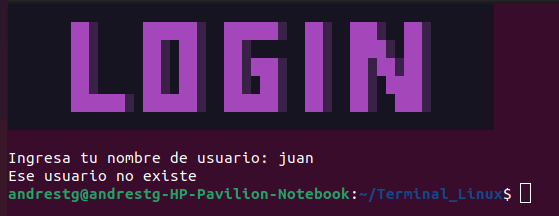
\includegraphics[scale=0.7]{imagenes/acceso.png}
\end{figure}
\begin{figure}[H]
	\centering
	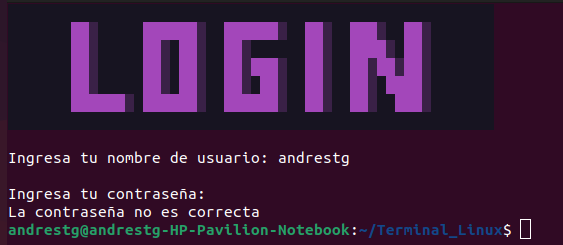
\includegraphics[scale=0.7]{imagenes/acceso2.png}
\end{figure}
\subsection{Línea de comandos}
\textbf{Explicación:} \par
El primer método de este script es \textquotedblleft permisos \textquotedblright, el cual lo único que hace es darle permisos de ejecución a todos los scripts que se podrían ejecutar con los comandos que implementamos.\\
\vspace{\baselineskip}

Después sigue el método \textquotedblleft titulobonito \textquotedblright que implementa los ascii arts de la terminal.\\
\vspace{\baselineskip}

Lo siguiente que se realiza es reescribir el método \textquotedblleft clear \textquotedblright, de manera que ahora no sólo limpiará la terminal, sino que además volverá a imprimir el título bonito.\\
\vspace{\baselineskip}

Posteriormente, en la línea 25 se implementa el \textquotedblleft trap \textquotedblright para que no sea posible salir de la terminal haciendo uso de ctrl+C y ctrl+Z, ya que en lugar de funcionar como normalmente lo harían, ahora indicarán que no es posible salir de la terminal de esa forma. Al final del código, en la línea 47, se regresa el comportamiento de estos comandos al normal.\\
\vspace{\baselineskip}

En el mismo sentido, se reescribe el comando \textquotedblleft exit \textquotedblright para que tampoco sea posible salir de la terminal con este comando.\\
\vspace{\baselineskip}

Terminando de explicar los métodos, el código es básicamente un while eterno del que solo se puede salir si se introduce el comando \textquotedblleft salir \textquotedblright; lo que se realiza en este bucle es leer el comando introducido por el usuario, verificar si existe el archivo homónimo al agregarle la extensión \textquotedblleft .sh \textquotedblright y verificar que no se trate del comando de acceso (ya que acceder a punk.sh desde la misma punk.sh podría causar problemas). Si el ejecutable existe, se ejecuta desde el contexto de esta shell, si no existe, usando \textquotedblleft eval \textquotedblright se solicita que se ejecute la línea introducida directamente en la terminal original (para que funcionen los comandos nativos de esta shell).\\
\vspace{\baselineskip}

\textbf{Código:} \par
\begin{lstlisting}[style=BashInputStyle]
#!/bin/bash
/usr/bin/clear
#Le da permisos a todos los .sh del proyecto
permisos(){
    chmod +x ayuda.sh
    chmod +x creditos.sh
    chmod +x juego.sh
    chmod +x time.sh
    chmod +x musica.sh
    chmod +x buscar.sh
    chmod +x infosis.sh
}

titulobonito(){
    ...
}

#Para que el título bonito siga saliendo
clear(){
    /usr/bin/clear
    titulobonito
}

#Para evitar que se pueda salir con ^Z,^C y exit
trap ... SIGINT SIGTSTP
exit() {
    echo "Eso no funcionará"
    echo ""
}

permisos
titulobonito
while true; do
    echo -n -e "\e[32m$USER:\e[0m \e[31m~$(basename "$PWD") > \e[0m"
    read comando
    if [ "$comando" == "salir" ]; then
        break
    fi
    #ejecuta el comando si existe el archivo con .sh, exceptuando access.sh
    if [ -e "$comando.sh" ] && [ "$comando" != "punk" ]; then
	. "./$comando.sh"
    else
        eval $comando
    fi
done

trap - SIGTSTP SIGINT SIGTERM
\end{lstlisting}
\vspace{\baselineskip}

\textbf{Ejecución:} \par
\begin{figure}[H]
	\centering
	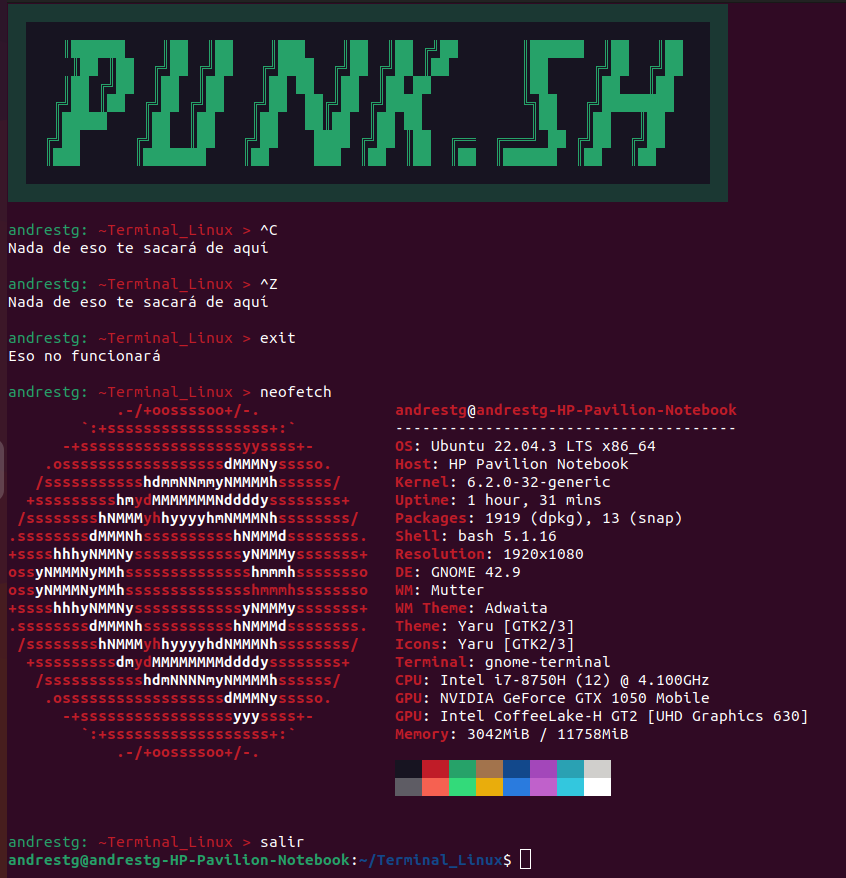
\includegraphics[scale=0.5]{imagenes/cli.png}
\end{figure}
\newpage
\subsection{Ayuda}
Este script solo es un conjunto de impresiones.\\
\textbf{Ejecución:}\par
\begin{figure}[H]
	\centering
	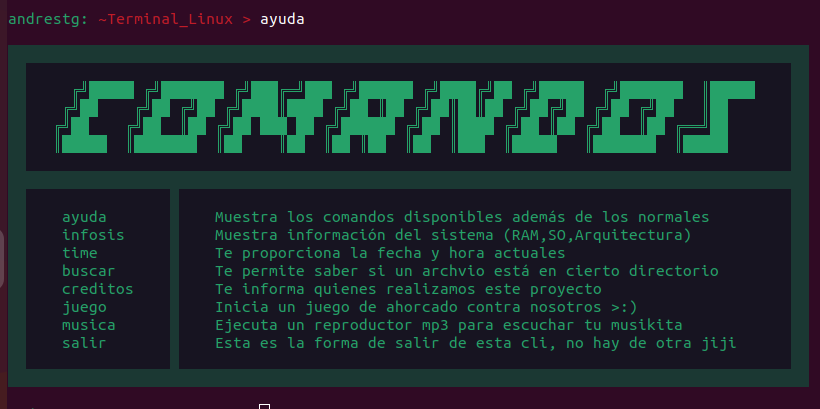
\includegraphics[scale=0.6]{imagenes/ayuda.png}
\end{figure}
\subsection{Información del sistema}
\textbf{Explicación:}\par
\vspace{0.3cm}
El diseño se enfoca en neofetch, por lo cual se tuvo que buscar en dónde se almacena cada información requerida, que en este caso, se tenga el usuario, nombre de computadora, OS, host, memoria del sistema, kernel, shell y CPU. 
\begin{itemize}
    \item Usuario: se requirió del comando \textit{whoami} para indicar el usuario en sesión.
    \item Nombre de computadora: El nombre se puede encontrar fácilmente al ingresar el comando \textit{hostname} el cual regresa lo necesitado.
    \item OS: Para el OS se requiere saber el sistema operativo, la distribución y la arquitectura.
    \begin{itemize}
        \item Sistema operativo: este se obtiene del comando \textit{uname} y la bandera \textit{-o}.
        \item Distribución: hay un archivo que se llama \textit{os-release} que guarda esta información, solo es cosa de usar \textit{grep} para obtener en específico esta informacióny después acortar la cadena dada.
        \item Arquitectura: esta se puede obtener con el comando \textit{uname} y bandera \textit{--machine}.
    \end{itemize}
    \item Host: Para obtener toda la información, se usa el comando \textit{hostnamectl} que ofrece toda esta información, como la marca, modelo y version.
    \begin{itemize}
        \item Marca: se obtiene una subcadena de \textit{Hardware Vendor}
        \item Modelo: se obtiene una subcadena de \textit{Hardware Model}
        \item Version: se obtiene una subcadena de \textit{Firmware Version}
    \end{itemize}
    \item Memoria del sistema: Para la memoria, se necesita saber el total y lo usado, ambos se pueden obtener con \textit{free} y para la medida de tamaño se usa la bandera \textit{--mega} la cual nos da la información en Megabytes.
    \begin{itemize}
        \item Total: se obtiene una subcadena de la subcadena de \textit{Mem}.
        \item Usado: se obtiene una subcadena de la subcadena de \textit{Mem}.
    \end{itemize}
    \item Kernel: El comando \textit{uname} con bander \textit{-r} devuelve esa información.
    \item Shell: La variable de entorno \textit{\textdollar SHELL} contiene esa información, solo se obtiene la subcadena de \textit{version}.
    \item CPU: Se obtiene toda la información del archvo \textit{cpuinfo} y se obtiene la cadea de \textit{model name}.
\end{itemize}
\textbf{Código:} \par
\begin{lstlisting}[style=BashInputStyle]
#!/bin/bash


#SISTEMA OPERATIVO
arq_sis=$(uname --machine) #ARQUITECTURA
distro=$(cat /etc/os-release | grep PRETTY_NAME)
distroBien=${distro:12} #SISTEMA OPERATIVO

#Host modelo de compu
manufacturer=$(hostnamectl | grep "Hardware Vendor")
man=${manufacturer:18}
productName=$(hostnamectl | grep "Hardware Model")
product=${productName:18}
version=$(hostnamectl | grep "Firmware Version")
ver=${version:18}

#Mem: total used free shared buff/cache available
meminfo=$(free --mega | grep Mem) #Obtiene información de la ram en MB

ram_total=${meminfo:15:5} #se obtiene subcadena de la cadena de meminfo sobre el total
ram_used=${meminfo:27:5} #se obtiene subcadena de la cadena de meminfo sobre el usado

#KERNEL
#echo "Kernel: $(uname -r)"

#Shell
shell=$SHELL
shellver=$(${shell:5} --version | grep version)
pos=$(expr index "$shellver" "version")-1
versionsh=${shellver:$pos+12:6}

#CPU
modelname=$(grep "model name" /proc/cpuinfo | uniq)
cpu=${modelname:13}

#IMPRESION DEL INFOSIS
...$(whoami)@$(hostname)...
...$(uname -o) $distroBien $arq_sis...
...$man $product $ver...
...$ram_used MB / $ram_total MB...
...$$(uname -r)...
...$versionsh...
...$cpu...

\end{lstlisting}

\textbf{Ejecución:} \par
\begin{figure}[H]
	\centering
	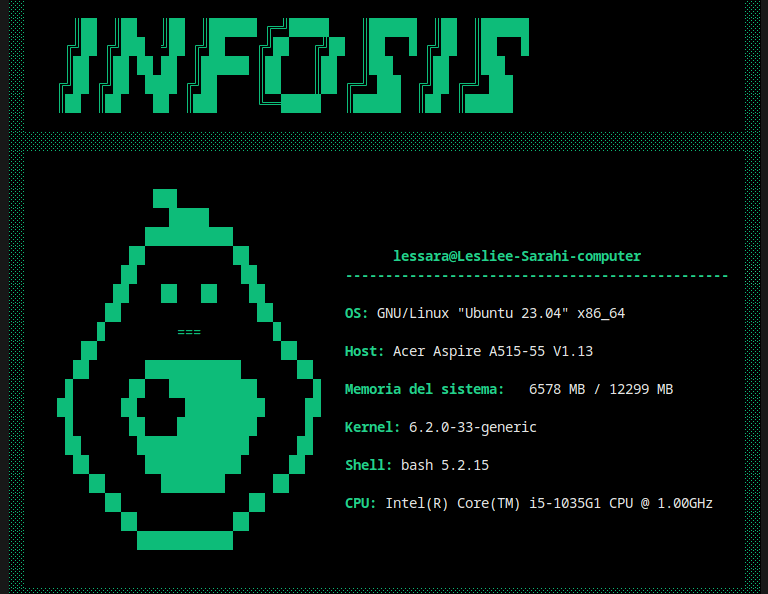
\includegraphics[scale=0.6]{imagenes/infosis.png}
\end{figure}

%\newpage
\subsection{Fecha y Hora}
\textbf{Explicación:} \par
\vspace{0.3cm}
Para hacer conocer la fecha y hora, se cuenta con archivos RTC, los cuales nos proporcionan información en tiempo real de ambos. Para conocer su información, se hace uso del comando \textit{cat}. Sin embargo, para que salga la hora local del sistema en el reloj, se tienen que hacer modificaciones ya que el reloj RTC tiene como default la zona horaria UTC, la cual no es mucha ayuda si no te encentras en esa zona. Es por lo cual, se agrega un comando antes de esto el cual nos cambia la ora RTC por la hora local que tenga el dispositivo.
\\\\
\textbf{Código:} \par
\begin{lstlisting}[style=BashInputStyle]
#!/bin/bash

#Ruta /sys/class/rtc/rtc contiene archivos de fecha y hora. Sin embargo, la hora está establecida en utc

timedatectl set-local-rtc 1 #Set el reloj as local time

date=$(cat /sys/class/rtc/rtc0/date)
hora=$(cat /sys/class/rtc/rtc0/time)


echo -e "\e[40m\e[32m\033[1mFECHA: $date                                                     \033[0m\e[0m" 
echo -e "\e[40m\e[32m\033[1mHORA: $hora                                                        \033[0m\e[0m" 
printf "\n"
\end{lstlisting}
\textbf{Ejecución:} \par
\begin{figure}[H]
	\centering
	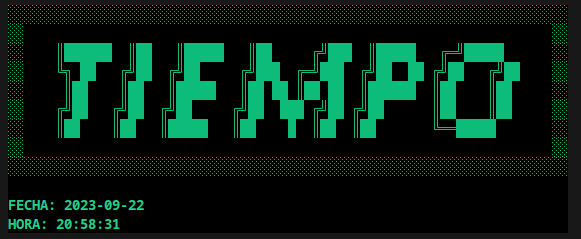
\includegraphics[scale=0.7]{imagenes/time.png}
\end{figure}

\subsection{Búsqueda de archivo}
\textbf{Explicación:} \par
\vspace{0.3cm}
Para hacer la búsqueda de un archivo dado el nombre del archivo y la carpeta, se requiere pedir ambos al usuario. Para verificar la existencia de la carpeta y del archivo se necesita de su ruta absoluta, tanto del directorio como del archivo. Para la ruta del directorio se junta la variable de entorno \textit{\textdollar HOME} y el nombre de la carpeta para formar la ruta, mientras que para la ruta del archivo, se concatena la ruta del directorio con y el nombre del archivo. Ahora bien, para la verificación de la existencia de ambos se hace uso del condicional \textit{if else} con sus respectivos operandos, \textit{-d} para la carpeta y \textit{-e} para el archivo. En caso de que exista la carpeta, entonces hará la búsqueda del archivo con la condicional, y si se encuntra, muestra en pantalla que sí está dentro de la carpeta, en caso erróneo mostrará que no se encuentra, así mismo para el caso de que no exista la carpeta dada.\\
\newpage
\textbf{Código:} \par
\begin{lstlisting}[style=BashInputStyle]
#!/bin/bash

logo(){
    ...
}

ingresarDatos(){
    echo -e "\e[31m\033[1mNOTA:\033[0m \e[32mSu carpeta se debe encontrar en guardada en el usuario actual\e[0m"
    printf "\e[32m\033[1mIngrese la carpeta donde cree que se encuentra su archivo: \e[0m"
    printf "\e[32m"
    read carpeta
    printf "\033[1mIngrese el nombre del archivo a buscar: \e[0m"
    printf "\e[32m"
    read archivo
    directorio=$HOME/$carpeta
    rutaArchivo=$directorio/$archivo
}

#Busqueda de carpeta 
busqueda(){
    if [ -d $directorio ]; then
        #Busqueda del archivo
        if [ -e $rutaArchivo ];then
            echo -e "\e[34m\033[1mEl archivo '$archivo' sí se encuentra en la carpeta '$carpeta'\e[0m"  
        else
            echo -e "\e[31m\033[1mEl archivo '$archivo' no se encuentra en la carpeta '$carpeta'\e[0m"
        fi  
    else 
        echo -e "\e[31m\033[1mLa carptea '$carpeta' no existe\e[0m"
    fi
}

main(){
    logo
    ingresarDatos
    echo ""
    busqueda
}

main
\end{lstlisting}
\newpage
\textbf{Ejecucuiones:} \par

\begin{figure}[H]
	\centering
	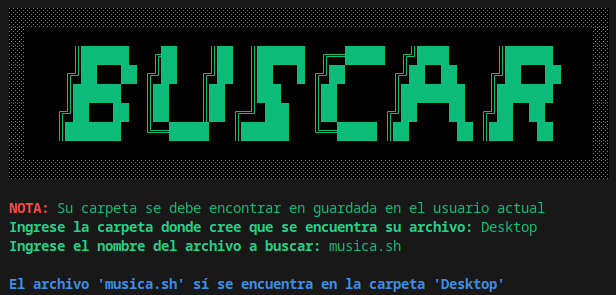
\includegraphics[scale=0.65]{imagenes/buscar1.png}
\end{figure}
\begin{figure}[H]
	\centering
	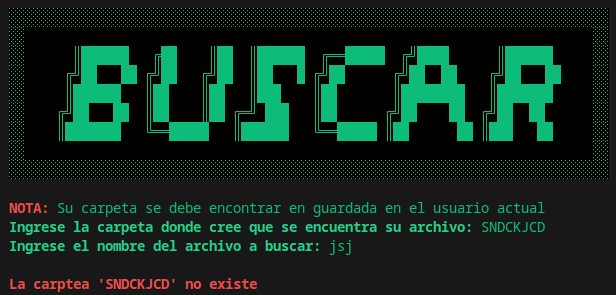
\includegraphics[scale=0.65]{imagenes/buscar2.png}
\end{figure}
\begin{figure}[H]
	\centering
	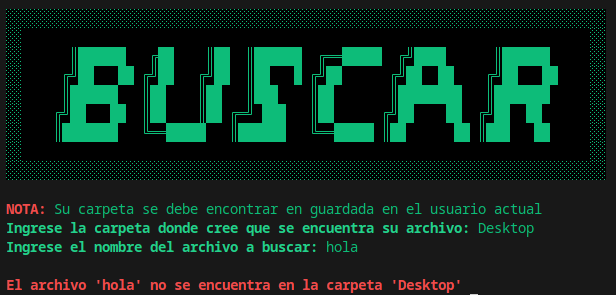
\includegraphics[scale=0.65]{imagenes/buscar3.png}
\end{figure}

\subsection{Créditos}
Este script solo es un conjunto de impresiones.\\
\textbf{Ejecución:} \par

\begin{figure}[H]
	\centering
	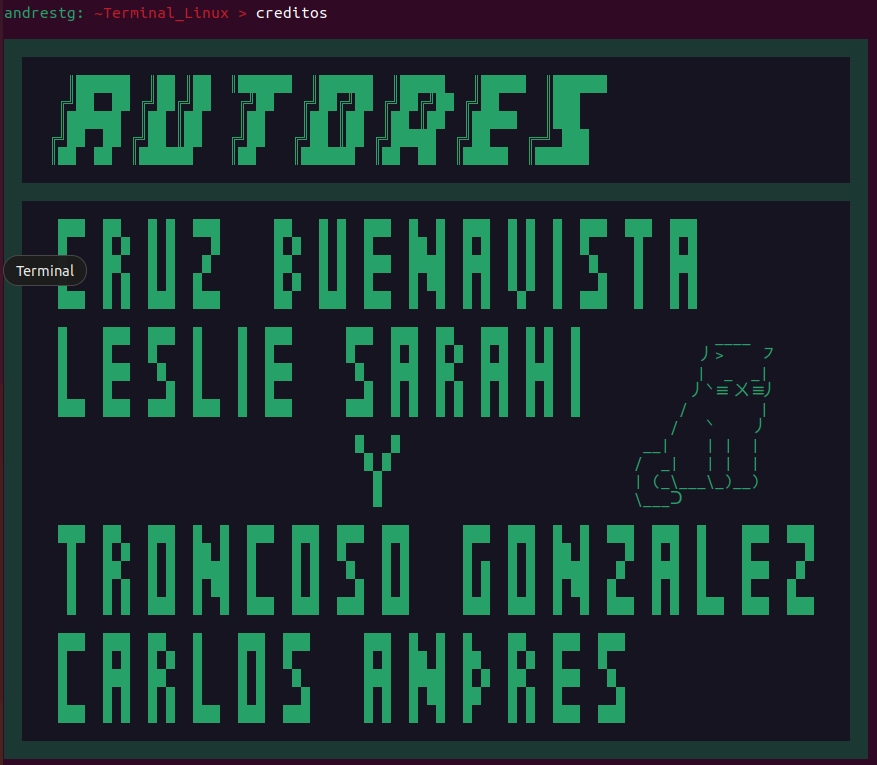
\includegraphics[scale=0.6]{imagenes/creditos.png}
\end{figure}

\textbf{Capturas:} \par

\subsection{Juego (Ahorcado)}
\textbf{Explicación:} \par
Lo más complejo de este código es la forma en la que emula un arreglo de mapas de arreglos, ya que en Shell solo es posible crear arreglos de valores, no de variables. Por ello, al principio de la ejecución se inicializa el arrelgo \textquotedblleft categorias\textquotedblright, el cual es un arreglo de strings, cada una de las strings, contiene internamente una string con la inicialización de un \textquotedblleft subarreglo\textquotedblright (por lo que que las comillas que use este subarreglo se tienen que escapar para distinguirlas de las comillas del arreglo principal). Esto se seguirá tratando más adelante.\\
\vspace{\baselineskip}

Posteriormente, se le solicita al usuario la categoría en la que quiere jugar, y esta entrada se manda como argumento a la función \textquotedblleft juegar\textquotedblright.\\
\vspace{\baselineskip}

Lo primero que realiza esta función es iterar sobre las strings en el arreglo \textquotedblleft categorias\textquotedblright, de forma que para cada una de las strings, usa \textquotedblleft eval\textquotedblright para ejecutarlas en la terminal como si fueran comandos, lo cual hace que ahora sí se inicialicen realmente los \textquotedblleft subarreglos\textquotedblright de \textquotedblleft categorias \textquotedblright.\\
\vspace{\baselineskip}

Una vez hecho esto, es necesario acceder al arreglo de la categoría elegida, por lo que en la línea 7 se accede a la string con la inicialización del arreglo correspondiente, y se \textquotedblleft corta\textquotedblright, quedándonos con la parte previa al signo de igual; es decir, el nombre del subarreglo correspondiente a la categoría elegida.\\
\vspace{\baselineskip}

Luego, se genera un índice aleatorio, el cual se usa para escoger la palabra que saldrá. A continuación aparece la línea 11, la cuál considero que es la línea más compleja de comprender de todo este código. En esta línea, se solicita a la terminal que ejecute la string con el nombre del arreglo a usar, seguido de corchetes que contienen el índice generado aleatoriamente; la salida de esto será la palabra elegida, por lo que se almacena. Lo complejo de esta línea es entender el proceso y la sintaxis de la misma, ya que primeramente se realizan cambios a la string a ejecutar en terminal, cambiando la variable \textquotedblleft categoría\textquotedblright por el valor que almacena (el nombre del subarreglo al que se quiere acceder), y cambiando la variable recibida como primer argumento al valor que almacena la misma; sin embargo, se requiere escapar el primer \$, ya que se requiere que ese se ejecute en terminal para que la sintaxis de acceso a esa posición del arreglo sea correcta.\\
\vspace{\baselineskip}

En otras palabras, la string con el nombre del arreglo se está utilizando como si fuera tal cual el arreglo; \textbf{esta sentencia es tan poderosa que se podría usar para pedirle al usuario el nombre de las variables que se usarán en el código.}\\
\vspace{\baselineskip}

Posteriormente se crea la palabra que le aparecerá al usuario (incialmente con puros guiones bajos), por lo que usando un for que recorre la palabra de respuesta, se agregan guiones bajos a cualquier caracter que aparezca exceptuando el espacio, caso para el cual se le agregara el mismo espacio.\\
\vspace{\baselineskip}

Después, el códio entra en un bucle eterno, el cual inicia dibujando el estado actual del juego con el método correspondiente, mandándole como argumento el estado actual del juego. A continuación se checa si este estado es 6, es decir, si el usuario ya cometió los errores máximos, en dado caso, se consulta si el usuario quiere volver a jugar (en cuyo caso el script hace una recursión), y se termina el programa. En caso de que el usuario aún no haya perdido, se le solicita un caracter. Posteriormente se recorre la palabra actual, de forma que cada vez que la palabra actual tiene el mismo caracter que la respuesta, se anota el acierto; cuando no coincide, se evalúa si coincide con el caracter ingresado, si esto se cumple se anota como un nuevo acierto que se realizo con esa jugada. Terminando de recorrer la palabra, se evalúa si el total de aciertos y aciertos nuevos es igual a la longitud de la respuesta, ya que en este caso el usuario ya ganó; por lo que se imprime la pantalla de ganador, se consulta si se quiere jugar de nuevo (en cuyo caso el script realiza una recursión), y se termina el programa. Si el usuario aún no gana, se verifica si hubo alguna nueva coincidencia, si no hubo, el número de errores aumenta.\\

\textbf{Código:} \par
\begin{lstlisting}[style=BashInputStyle]
#!/bin/bash
juegar(){
    #crear e inicializar los "subarreglos"
    for elt in "${categorias[@]}";do eval $elt;done
    
    #Adquirir el nombre del subarreglo
    categoria=$( echo ${categorias[$1]} | cut -d "=" -f1 )

    #Escoger una de las palabras aleatoriamente
    ind=$(($RANDOM%20))
    respuesta=$(eval echo "\${${categoria}[$ind]}") #Para usar el string con el nombre del arreglo como el arreglo, y acceder a la posición
    
    #Hacer la palabra oculta
    palabra=()
    for i in $(seq 0 $((${#respuesta}-1 ))); do
        #Si es espacio, da un output quejándose por el !=, por eso lo envío a /dev/null
        if [ ${respuesta:$i:1} != " " &>/dev/null ]; then
            palabra+=("_")
        else
            palabra+=(" ")
        fi 
    done
    #iterar sobre los intentos
    i=1
    while true ; do
        dibujo $i $1
        #Checa si ya perdiste
        if [ $i -eq 6 ]; then
            read -p "Presiona enter para continuar, \"1\" para jugar otra vez: " enter
            if [ $enter -eq 1 &>/dev/null ]; then
                source juego.sh
            fi
            return
        fi

        read -p "Ingresa un caracter (todas las letras deben ser mayúsculas): " caracter
        aciertos=0
        aciertosNuevos=0
        #comparar la palabra y el nuevo caracter con la respuesta
        for ((j=0; j<${#palabra[@]}; j++ )); do
            #La segunda condición es porque tiene problemas para comparar los espacios
            if [ ${palabra[j]} != ${respuesta[@]:$j:1} ] && [ ${respuesta[@]:$j:1} != " " &>/dev/null ]; then
                #Los /dev/null es porque da una salida quejándose por el uso del == y !=
                if [ $caracter == ${respuesta[@]:$j:1} &>/dev/null ]; then
                    palabra[j]=$caracter
                    ((aciertosNuevos++))
                fi
            else
                aciertos=$((aciertos+1))
            fi
        done

        #Verifica si ya ganaste
        if [ $(($aciertos + $aciertosNuevos)) -eq ${#respuesta} ]; then
            /usr/bin/clear
            ...
            ...
            read -p "Presiona enter para continuar, \"1\" para jugar otra vez: " enter
            if [ $enter -eq 1 &>/dev/null ]; then
                source juego.sh
            fi
            return
        fi

        #Verifica si hubo avances
        if [ $aciertosNuevos -eq 0 ]; then
            i=$((i+1))
        fi
    done
    echo "perdiste"

}

dibujo(){
    ...
}

pista=( "DISTRIBUCION DE LINUX" "LENGUAJE DE PROGRAMACIÓN" "BECARIO DE PROTECO" "FACULTAD/ESCUELA" "MATERIA DE ING.COMPUTACIÓN" "CIUDAD")
categorias=(
    "distros=( \"DEBIAN\" \"FEDORA\" \"REDHAT\" \"UBUNTU\" \"ARCH\" \"KALI\" \"ORACLE\" \"MINT\" \"LITE\" \"MANJARO\" \"ELEMENTARY\" \"DEEPIN\" \"HANNAH MONTANA\" \"TURBO\" \"KNOPPIX\" \"CENTOS\" \"MANDRIVA\" \"SUSE\" \"GENTOO\" \"SLACKWARE\")"
    "lenguajes=( \"R\" \"C#\" \"C++\" \"C\" \"PYTHON\" \"JAVA\" \"JAVASCRIPT\" \"JULIA\" \"POSTGRESQL\" \"ELIXIR\" \"MATLAB\" \"PHP\" \"RUBY\" \"SWIFT\" \"KOTLIN\" \"GO\" \"SHELL\" \"PERL\" \"PASCAL\" \"COBOL\")"
    "becarios=( \"BRIAN\" \"PAMELA\" \"ABRAHAM\" \"JAVIER\" \"EITHAN\" \"LEONARDO\" \"DEIVI\" \"JOHN\" \"ALEJANDRO\" \"PAULA\" \"ALBANYA\" \"MARTIN\" \"CHILPA\" \"ENFRIJOLADA\" \"SAMUEL\" \"ATHENAS\" \"ALAN\" \"JIMENA\" \"CYNTHIA\" \"JON\")"
    "facultades=( \"INGENIERIA\" \"PSICOLOGIA\" \"MEDICINA\" \"CIENCIAS\" \"DERECHO\" \"ECONOMIA\" \"ARTE Y DISEÑO\" \"FILOSOFIA\" \"POLITICAS Y SOCIALES\" \"VETERINARIA\" \"CONTADURIA Y ADMINISTRACION\" \"ARQUITECTURA\" \"MUSICA\" \"QUÍMICA\" \"FES IZTACALA\" \"FES ARAGON\" \"FES ZARAGOZA\" \"FES ACATLAN\" \"FES CUAUTITLAN\" \"ODONTOLOGIA\")"
    "materias=( \"EDA\" \"POO\" \"SEÑALES Y SISTEMAS\" \"BASES DE DATOS\" \"MATEMATICAS AVANZADAS\" \"ALGEBRA LINEAL\" \"CALCULO VECTORIAL\" \"INTELIGENCIA ARTIFICIAL\" \"SISTEMAS OPERATIVOS\" \"ESTRUCTURAS DISCRETAS\" \"REDES DE DATOS\" \"MECANICA\" \"ANALISIS NUMERICO\" \"PROBABILIDAD\" \"REDACCION\" \"ECONOMIA\" \"FINANZAS\" \"ETICA\" \"ECUACIONES DIFERENCIALES\" \"CIRCUITOS ELECTRICOS\")"
    "ciudades=( \"ROMA\" \"MENDOZA\" \"PORTLAND\" \"BERLIN\" \"CHICAGO\" \"ERITREA\" \"LIMA\" \"SANTIAGO\" \"KUALA LUMPUR\" \"EL CAIRO\" \"MADRID\" \"BARCELONA\" \"NUEVA DELHI\" \"PORTO\" \"MOSCU\" \"TOKIO\" \"QUEBEC\" \"SEUL\" \"PRAGA\" \"HONG KONG\")"
)

...
echo -n "NÚMERO DE LA OPCIÓN ELEGIDA: "
read opcion

opcion=$((opcion-1))
if [ $opcion -lt  6 ]; then
    juegar $opcion 
else
    clear
fi

\end{lstlisting}
\textbf{Ejecuciones:} \par
\begin{figure}[H]
	\centering
	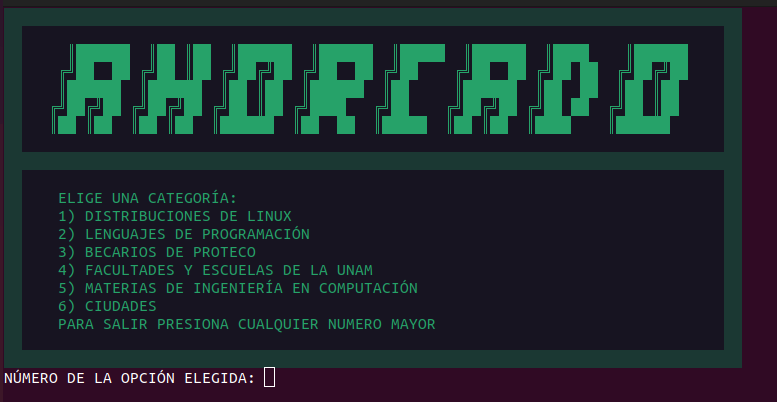
\includegraphics[scale=0.6]{imagenes/ahorcado.png}
\end{figure}
\begin{figure}[H]
	\centering
	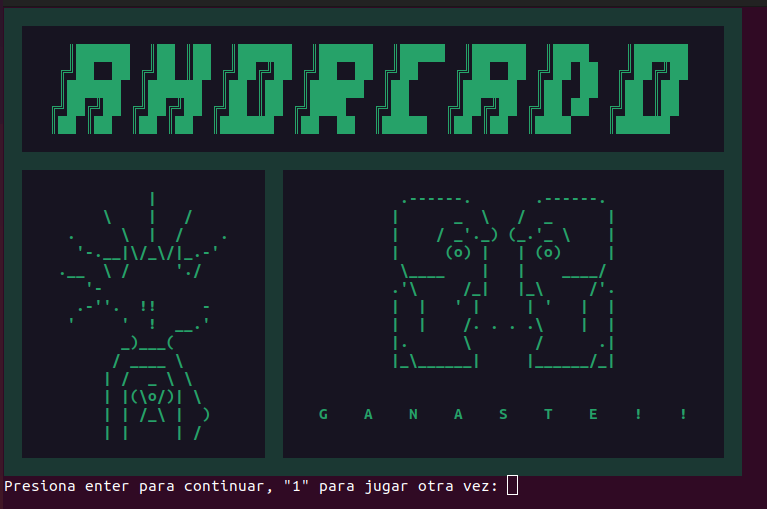
\includegraphics[scale=0.6]{imagenes/ahorcado1.png}
\end{figure}
\begin{figure}[H]
	\centering
	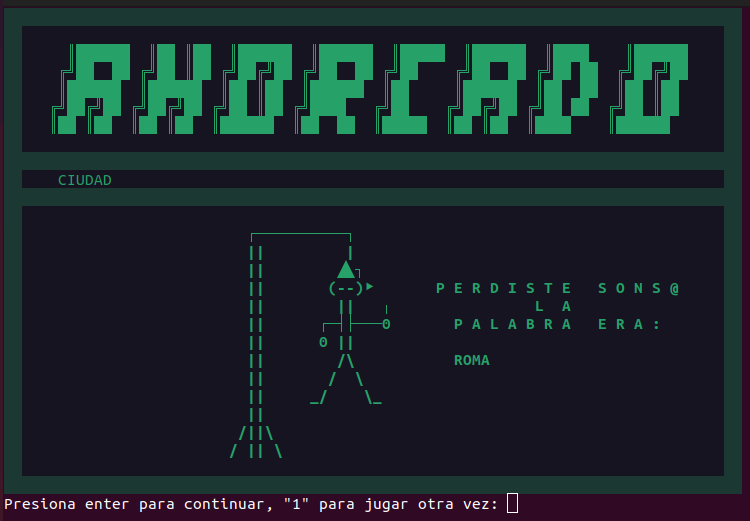
\includegraphics[scale=0.6]{imagenes/ahorcado2.png}
\end{figure}
\begin{figure}[H]
	\centering
	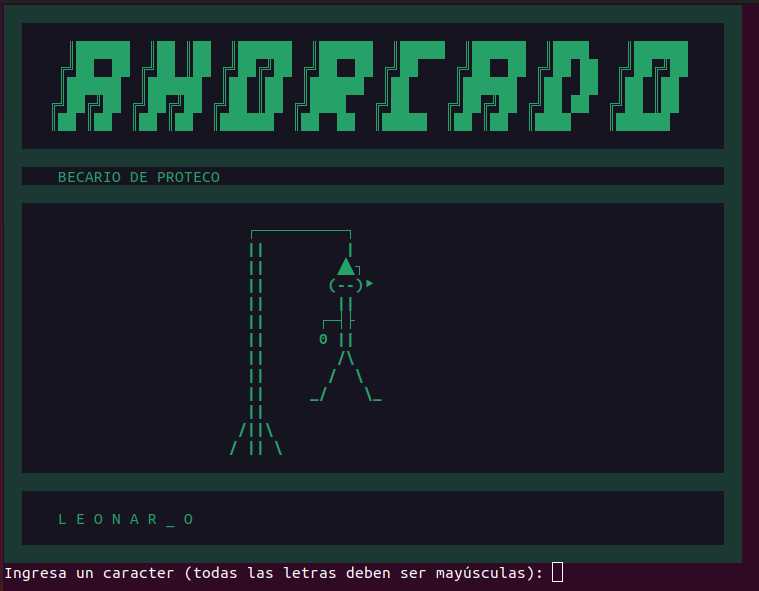
\includegraphics[scale=0.6]{imagenes/ahorcado3.png}
\end{figure}
\subsection{Reproductor MP3}
\textbf{Explicación:} \par
\vspace{0.3cm}
En primera instancia, el programa va a verificar la existencia del programa, para ello, se usa el comando which para indicar si se encuentra, si regresa información, entonces se encuentra instalado, si no, le pide al usuario si lo quiere o no instalar. Luego, se le pide al usuario que ingrese una ruta donde se encuentre archivos mp3, esos archivos mp3 los busca y los cuarda en un archivo con extensión m3u, que es un tipo de acrhivo que guarda playlist. Para repoducir canciones, el usuario tiene dos opciones, o reproducir una única canción o toda la playlist. Para reproducir una única canción, se mapea el archivo mp3 y se imprime las posibles opciones al usuario, donde el puede escoger qué canción quiere. En el caso de que se quiera toda la playlist, se reproduce el archivo m3u con ayuda de la bandera \textit{@} que nos permite escuchar todas las canciones de cierto archivo. Para ambos casos, el programa mpg123 da como salida información, entonces para que no lo muestre, se hace uso de la bandera \textit{q}. Finalmente, para que el usuario pueda controlar la música, se hace uso de las teclas que el mismo mpg123 ofrece y solo se imprimen los más importantes o esenciales de un reproductor.\\ 
\newpage
\textbf{Código:} \par
\begin{lstlisting}[style=BashInputStyle]
#!/bin/bash

#logo
logo(){
    ...
}

#Verificación de instalación de mpg123
verificacion(){
    if  which mpg123 &> /dev/null; then #&> sirve para redirigir salidas estandar y error
        echo "Está instalado, no es necesario su instalación"
    else
        echo "NO SE ENCUENTRA INSTALADO EL PROGRAMA"
        printf "¿Desea instalarlo para continuar con la reproducción [yes/no]?: "
        read opcion
        opcion=$(echo "$opcion" | tr '[:upper:]' '[:lower:]') #en caso de mayusculas las cambia a minusculas
        if [ $opcion == "yes" ]; then
            echo "NOTA: Solo se instalará si la distribución del dispositivo está basada en debian"
            sudo apt install mpg123
        elif [ $opcion == "no" ]; then
            echo "No se podrá instalar"
            exit
        else
            echo "No es una opción válida"
        fi
    fi
}

comprobrarCanciones(){
    echo "Ingrese la ruta donde se encuentre su carpeta de música: "
    read ruta
    if [ -d $ruta ]; then
        canciones="canciones.m3u" #extensión para playlists
        find "$ruta" -type f -name "*.mp3" > "$canciones"
        if [ ! -s "$canciones" ]; then
            echo "No hay canciones en esta carpeta"
        fi
    else
        echo "La carpeta que ingreso no es válida"
    fi
}

menuCanciones(){
    ...
}
#menu de controles al estar reproduciendo musica
menuControl(){
    ...
}

reproducirTotal(){
    menuControl
    mpg123 -q -@ "$canciones" 

    rm -f "$canciones"
}

menuControlIndividual(){
    ...
}

reproduccionIndividual(){
    menuControlIndividual
    mapfile -t lista < "$canciones" #mapea las canciones del archivo m3u

    echo "Lista de canciones disponibles:"
    for i in "${!lista[@]}"; do
        echo "$i: ${lista[$i]}"
    done
    echo "Por favor, elija un número de canción para reproducirla:"
    read opcion

    # Verificar si la opción seleccionada es válida
    if [[ ! $opcion =~ ^[0-9]+$ || $opcion -lt 0 || $opcion -ge ${#lista[@]} ]]; then
        echo "Opción no válida. Por favor, seleccione un número válido."
        exit 1
    fi

    # Reproducir la canción seleccionada
    mpg123 -q "${lista[$opcion]}"
}


main(){
    clear
    opcion=0
    logo
    verificacion
    comprobrarCanciones
    
    while [ "$opcion" != 3 ]; do
        clear
        menuCanciones
        echo "Inserte opción: "
        read opcion
        case $opcion in
            1)                
                clear
                logo
                reproduccionIndividual
                ;;
            2)                
                clear
                logo
                reproducirTotal
                ;;
            3)    
                clear
                logo
                echo "Hasta luego! :)"    
                ;;
            *)    
                echo "Opción no valida"
                ;;
        esac
    done
    
}
main
\end{lstlisting}
\textbf{Capturas:} \par
\begin{figure}[H]
	\centering
	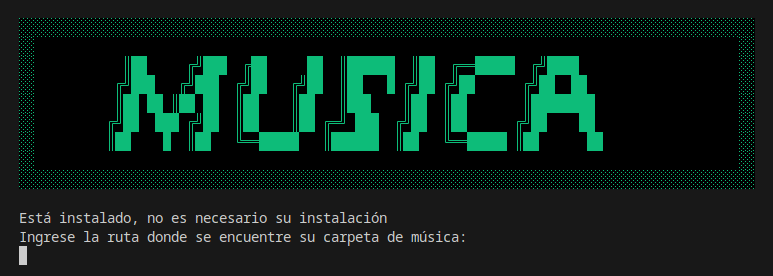
\includegraphics[scale=0.6]{imagenes/musica1.png}
\end{figure}
\begin{figure}[H]
	\centering
        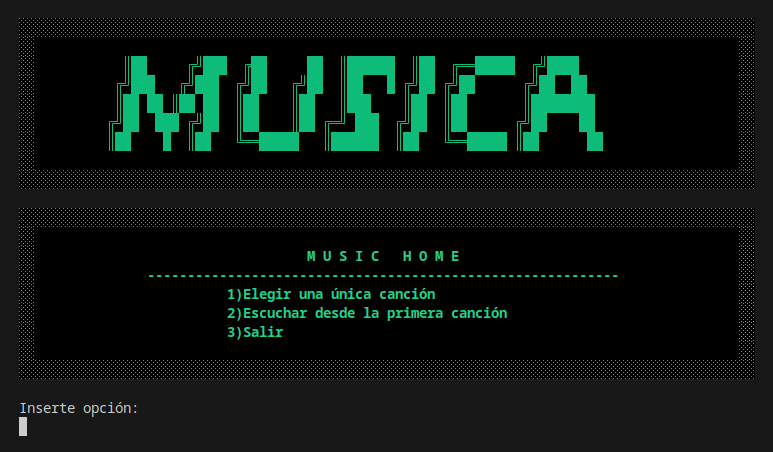
\includegraphics[scale=0.6]{imagenes/musica2.png}
\end{figure}
\begin{figure}[H]
	\centering
        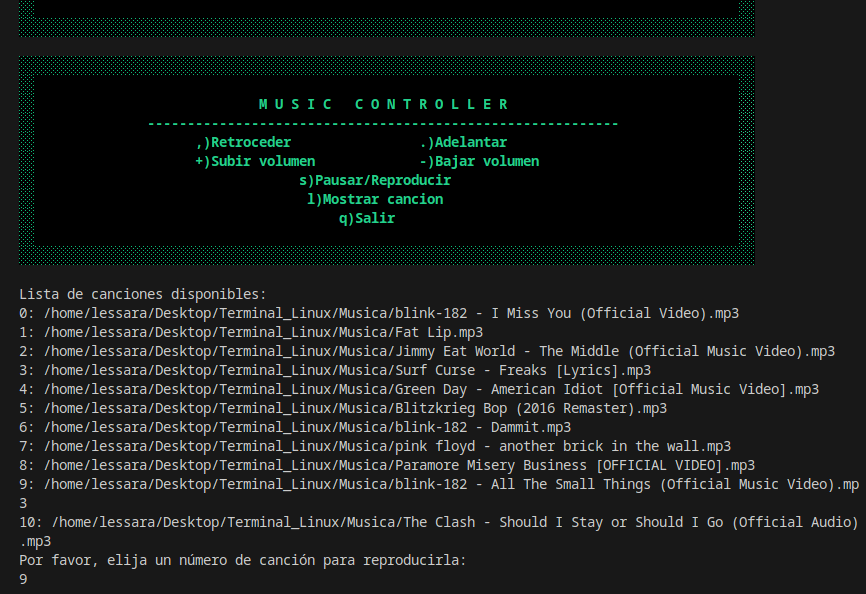
\includegraphics[scale=0.6]{imagenes/musica3.png}
\end{figure}
\begin{figure}[H]
	\centering
        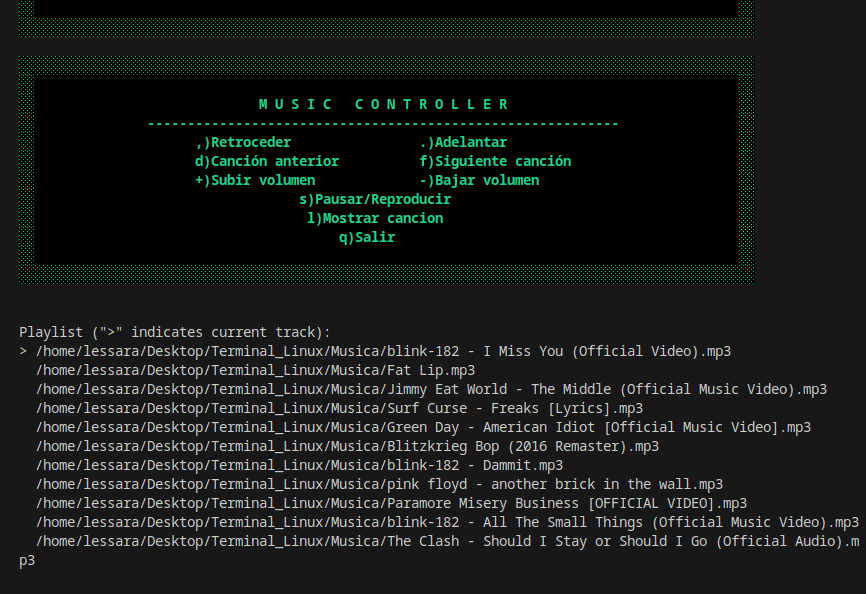
\includegraphics[scale=0.6]{imagenes/musica4.png}
\end{figure}

\section{Conclusiones}
\subsection*{Cruz Buenavista Lesliee Sarahí:}
Con la realización del proyecto pude poner en práctica lo que estuvimos viendo durante el curso. Sin emabrgo, me costó un poco de trabajo, ya que no todo lo vimos en clase, por lo cual tuve que ser autodidacta para ciertos puntos y de esta forma cumplir con lo requerido.
\\\\

Algo que me gustó de este proyecto, es que aprendí cosas que no sabía que se podían hacer. Tales  como hacer caso omiso a la salida que te da un comando, hacer subcadenas de cadenas, cambiar color de la salida de la terminal, aprender nuevas banderas, nuevos comandos, identificar archivos que guardan cierta información y saber cómo extraer algo en específico, 'jugar' con la entrada que da el usuario, entre otras cosas. Por otra parte, hubo sus complicaciones, ya que todo esto no lo conocía, por lo cual tuve que investigar en varias plataformas y chat bots con inteligencia artifical las cuales me ofrecían información de banderas, comandos y sintaxis necesario para cada uno. Así mismo, la dificutlad de hacer pruebas de lo que puede servir o no, qué puedo modificar para que mi código sea más eficiente y tenga menos errores e identificar errores obtenidos. 
\\\\

Durante clase, se supo que en el sistema GNU/Linux, todo es un archivo, por lo cual, trabajar con archivos es algo muy importante para el lenguaje shell, ya que te permitirá hacer las cosas que desees. Sin embargo, esto no es muy sencillo, ya que se debe conocer dónde se encuentra cada cosa y su repercución al modificar, agregar o eliminar algo. En lo personal, aunque esto te permita hacer básicamente tu propia distribución, no es algo que cualquier persona lo pueda hacer. Tal como mi caso, ya que aunque conozca algo sobre este sistema operativo, no creo tener los suficientes conocimientos y habilidades para lograr hacer una distribución como \textit{Ubuntu}, \textit{Debian}, \textit{RedHat}, \textit{CentOS} y de este estilo.
\\\\
En general, creo que el proyecto tiene el suficiente nivel para conocer Shell y GNU/Linux. Aunque no se pudo ver mucho en dos semanas de clases, este proyecto te incentiva a ser autodidacta. Este hecho es muy importante, ya que en carreras de ingeniería, es muy importante ser autodidactas en muchos temas. Finalmente, puedo decir que este proyecto me gustó incluso si me exigió el aprender e investigar. 

\subsection*{Troncoso González Carlos Andrés:}
Durante el desarrollo de este proyecto, me dí cuenta que lo aprendido en el curso no era suficiente para realizar prácticamente ninguno de los puntos que el trabajo debería de cumplir, por lo que comprendí que el propósito de este proyecto es en realidad desarrollar mi capacidad de investigar, aprender, y analizar por mi cuenta; objetivos que considero logré cumplir ampliamente. 
\vspace{\baselineskip}

En esta travesía de desarrollar el proyecto, atravesé dificultades con distintos aspectos con los que nunca me había involucrado profundamente, el primero a mencionar es el trabajar con múltiples archivos del sistema en los cuales se almacenan datos de usuarios, contraseñas, configuraciones, etc. Ya que para el desarrollo de este proyecto me fue necesario utilizarlos, y combinarlos con una gran cantidad de comandos que no fueron vistos durante el curso, para poder así extraer información de ellos y realizar acciones relativamente complejas dentro del sistema.
\vspace{\baselineskip}

Otra de las dificultades que atravesé fue diseñar un estilo propio y performático (punk), involucrándome con realizar ascii arts desde cero, pasando por una gran cantidad de diseños y evolucionándolos hasta llegar al resultado final. A pesar de las dificultades, puedo decir que estoy muy contento con el resultado, y considero que la terminal es estética y refleja el performance que quería representar con ella.
\vspace{\baselineskip}

Finalmente, la última dificultad que quiero mencionar, es la constante investigación, así como la prueba y error, para averiguar qué cosas sí se pueden hacer en shell, y qué cosas no se pueden hacer (como lo son los arreglos bidimensionales). Teniendo que lidiar con una sintaxis a mi parecer compleja, en la que no termino de comprender cuando se tienen que usar ciertas formas, y cuando ciertas otras. Creo que el epítome de esto es la emulación de un arreglo de mapas de arreglos que realicé en el script del juego, la cual me tomó días de investigación, prueba y error, y problemas con sintaxis, para que al final fuera posible emular en shell algo que no se puede hacer. Además, esta emulación me llevó a descubrir la fortaleza del lenguaje, ya que descubrí que ahora, con él, podría realizar cosas que hasta donde llega mi conocimiento, no es posible hacer en ningún otro lenguaje de programación (como lo es pedirle al usuario los nombres de las variables que se utilizarán a lo largo del programa).\\ 
\end{document}